\documentclass[conference]{IEEEtran}
\IEEEoverridecommandlockouts
% The preceding line is only needed to identify funding in the first footnote. If that is unneeded, please comment it out.
%Template version as of 6/27/2024

\usepackage{cite}
\usepackage{amsmath,amssymb,amsfonts}
\usepackage{algorithmic}
\usepackage{graphicx}
\usepackage{textcomp}
\usepackage[hidelinks]{hyperref}
\usepackage{xcolor}
\def\BibTeX{{\rm B\kern-.05em{\sc i\kern-.025em b}\kern-.08em
    T\kern-.1667em\lower.7ex\hbox{E}\kern-.125emX}}
\begin{document}

\title{A Brief Survey of Machine Learning and Deep Learning for Optimizing the Efficiency of Tiered Memory Management}

\author{\IEEEauthorblockN{Josh Borthick}
\IEEEauthorblockA{\textit{Computer Science Department} \\
\textit{College of Natural and Applied Sciences}\\
\textit{Missouri State University}\\
Springfield, Missouri, United States \\
jlb8976s@missouristate.edu}
}

\maketitle

\begin{abstract}
    Machine learning (ML) has been used for automation and knowledge creation since the 1960s, 
    including in the world of algorithm analysis, prediction, and optimization.  More recently, 
    these benefits have been applied to tiered memory management (TMM) to automate the mastery of and optimize the accuracy, throughput, and energy savings of page replacement policies for distributed computing systems.  The benefits of ML for TMM are nearly limitless.  For example, imagine an operating system designed with not just one perfectly optimized memory management policy but an adaptive policy able to further perfect itself as more and newer data are presented.  Imagine this management system even applying different policies for different use cases!  A human team would need to painstakingly implement some wonderful algorithm and do it again and again for each needed policy, while an ML model could learn to do this, offering massive savings in time and money.  This paper will begin by briefly delving into the histories of ML and TMM, providing a review of the studied literature, and from there giving an overview of common algorithms and their comparative benchmarks.  Finally, it will end with the shortcomings of modern ML in the world of TMM. 
\end{abstract}

\begin{IEEEkeywords}
tiered memory management, distributed computing, machine learning, deep learning, algorithms.
\end{IEEEkeywords}

\section{Introduction}

Human ingenuity has no limits, but time does.  Given enough time, humans might well continue to
improve algorithms forever, but what about tomorrow, next week, or next year?  Can we do better? 
Machine learning is the answer.  There are some very unique and clever ways to make computers do
their jobs accurately and quickly, and machine learning can make this process even better. 

\subsection{Motivation}

Machine learning refers to an algorithm that can be optimized for a given task, usually after weights are given to train while crunching data.  Deep learning is machine learning with neural networks.  There are three main categories of machine learning and many different types of neural nets.  The three ML categories are supervised, unsupervised, and reinforced learning.  Sometimes, aspects of both supervised and unsupervised are combined to create a kind of fourth category.  There are many different reasons to specialize an ML application or system, depending on the needed optimization or prediction.  The focus of this paper is the algorithms and techniques, both ML and non-ML, used in memory management, especially those used for tiered memory management.  A brief review of various non-ML algorithms will serve as an introduction to the machine learning tools and techniques which utilize them, followed by statistics on how well they did.  Finally, references will follow a brief conclusion. 

\section{History of Machine Learning and Memory Tiering}

Before hierarchical storage management (HSM), people had to manually read data from one memory tier to another.  International Business Machines (IBM) first utilized tiered storage for their mainframes by manually placing primary production data on varying configurations of hard drives and magnetic tape, based on each one's access speed and archival lifespan [1]. 

HSM, also first used by IBM in 1978 on their IBM 3850 Mass Storage Facility, automates the movement of data between tiers.  Users no longer needed to know where data was stored or how to get it back, the automated system handled everything.  These days, HSM is most often used for deep archival storage, but its concept is alive in all computers with multiple stages and speeds of memory storage, such as the central processing unit (CPU) registers, cache, random access memory (RAM), and hard disk drives of home computers and mobile phones [2]. 

Solid state drives (SSDs) have existed in some form since the mid-1970s, but more modern SSDs, created with flash memory, were marketed as early as 1991.  This was the status quo till the invention of non-volatile memory-express (NVMe).  According to the 1.0e specification notes, version 1.0 was ratified on March 1, 2011 [3].  They use zoned namespaces to allow direct byte-addressability without a flash translation layer.  In dual in-line memory module (DIMM) form factors, the same used by RAM, CPUs can access NVMe directly, just like RAM, providing a new tier of persistent memory between RAM and classic SSDs in which to store pages of data and instructions.  NVMe provides considerably more memory space than standard RAM, and while it is not as fast as RAM, it is much faster than SSDs and has lower access latency.  This creates the perfect environment for tiered memory management [4]. 

\begin{figure}
    \centering
    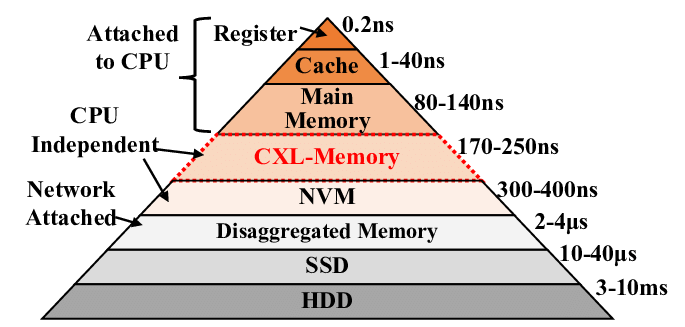
\includegraphics[scale=1.1]{tiering.png}
    \caption{Different tiers have different characteristics.}
\end{figure}

Now we have multiple tiers (above).  All processors have access to their individual registers and CPU-local cache, and they can all access dynamic random-access memory (DRAM), or “main memory” as listed in this image.  In this architecture, different CPUs working on the same machine are shown to have different non-uniform memory access (NUMA) to memory sets like Compute Express Link (CXL) memory or NVMe.  Any network(s) connected to a computer could have dedicated memory, and for most purposes, there must be some sort of permanent storage, noted here as an SSD and a hard drive disk (HDD). 

With all these types, physical and virtual locations, and latencies of memory and storage comes the need for rather complicated strategies, called policies, for managing the selecting, storing, and moving of data and instructions between tiers. 

\section{Non-ML Algorithms for Page (Re)placement}
Each policy has its own purpose—its own special benefit for why it should be selected for use in each situation or machine.  Benefits could include sheer simplicity of implementation and understanding, maximizing throughput of memory pages, minimizing the swapping out of often or recently used pages, or even the attempted prediction of patterns in commonly used data or of programmed loops.  Memory pages are collections of related data and instructions in sizes set by the kernel at compilation, often 4096 bytes.  Pages are usually strung together to hold information larger than 4096 bytes, and if those pages are not stored sequentially in physical or virtual memory—well, there are policies for managing that, as well.  Each policy also has its own drawbacks.  Where one policy’s algorithm is easy to use, it may be so easy at the expense of efficiency.  Another policy might be great at noticing patterns, making it amazing for high-throughput data science needs, but have a high swap-out rate, making it a poor choice for home computers or Web servers. 

Random page replacement, assuming that every page is as likely to be used again as every other page, is very easy to implement on most systems, but will randomly select hot pages to move to a lower, slower tier [6].  Those hot pages, pages with a higher access rate, will then need to be brought back into CPU-usable memory at the cost of the time necessary to swap them back to a faster tier or even to clear enough space to hold them.  First-in/first-out (FIFO) uses a queue to track a page’s access recency.  When brought into a tier, the page is placed into the back of the queue, and when memory needs freed, pages at the front of the queue are moved to slower memory or forgotten altogether.  This can be efficient for very small jobs or on systems with only one processor and thread but can require a page fault to retrieve a recently dismissed page in any loop involving more memory than can fit in the queue.  Least recently used (LRU) is much more complex, but also potentially much more efficient.  In a naive approach, lists of pages must be stored, sorted by recency, and searched for pages to evict from a memory tier.  Sorting and searching are computationally expensive, making it tricky to track page use recency.  Some mainframes and other systems have the kind of hardware built-in for tracking page features, making this approach feasible, but in other cases, naive LRU degrades performance. 

An alteration to naive LRU is to store and track a bit in each page.  On first finding a page in a list of eviction candidates, instead of evicting it, the page replacement algorithm sets this bit to represent that it has been passed over, once.  The next time the algorithm sees this page on searching the eviction-candidate list, it sees this bit already set and evicts the page from that tier.  This alteration to another algorithm is called second chance.  This and different techniques have been used to form useful algorithms or alterations to algorithms which improve their features.  Splitting a list by use frequency into two lists, having a special list of pages with exemptions protecting it from eviction, and setting tracking bits are common aspects of real-world policies in use in the world, today.   

Optimal page replacement is another algorithm, but it is infeasible in the real world since it requires foreknowledge of needed pages.  It is often useful for comparing realistic algorithms against one another when judged against this optimal possibility. 

These algorithms all play with the ideas of storing and tracking the features of pages like frequency and recency, using different data structures or turning bits on and off within each page.  Each individual algorithm is often cited by the name of the family of algorithms it belongs to, such as the FIFO (used for queues), last-in/first-out (LIFO, used for stacks), LRU, or LFU-based strategies.  But combinations and tweaks exist which can enhance any of these basic algorithms and make them better in all aspects than their previous incarnations. 

\section{Better Versions of Non-ML Algorithms}

Besides exception lists or splitting one queue into two based on access frequency, some techniques have found ways to make an algorithm self-tuning without adding overhead, like adaptive replacement cache (ARC), an IBM-proprietary algorithm which outperforms LRU in all aspects.  Clock, a version of LRU which serializes cache hits by using a single global lock, is an improvement on LRU and FIFO, but WSClock makes an extra check on each page as it sweeps the lists to see if the difference between the check time and the stored time is greater than some predetermined time slice.  In effect, it adds a check for frequency of last use.  If it is, that page is considered no longer important.  Clock with adaptive replacement (CAR) maintains two clocks, one for recency and one for frequency, each backed by LRU lists.  It is much better than LRU, Clock, or ARC, but is also patented by IBM.

\subsection{Multi-Clock}

Multi-Clock, created by Dr. Adnan Maruf of Missouri State University and Sylab of Florida International University, is open source (11).  It adds a third “promote” list to the second tier, shown below.  Multi-Clock adds to Linux’s LRU 2Q, which uses one active list and one inactive list per tier to track hot and cold pages.  If a page in a lower tier is used enough to be a candidate for moving to a higher tier, it is placed in the promote list.  Pages in the promote list are moved to the active list of a higher tier. Demotion is still accomplished via moving pages from a higher tier’s inactive list to the lower tier’s inactive list.  In this way, multi-clock tracks when pages have been accessed twice, finding hot pages with a lower overhead than is often associated with tracking use frequency.  Pages moved to a higher tier are more likely to be needed. 

\begin{figure}
    \centering
    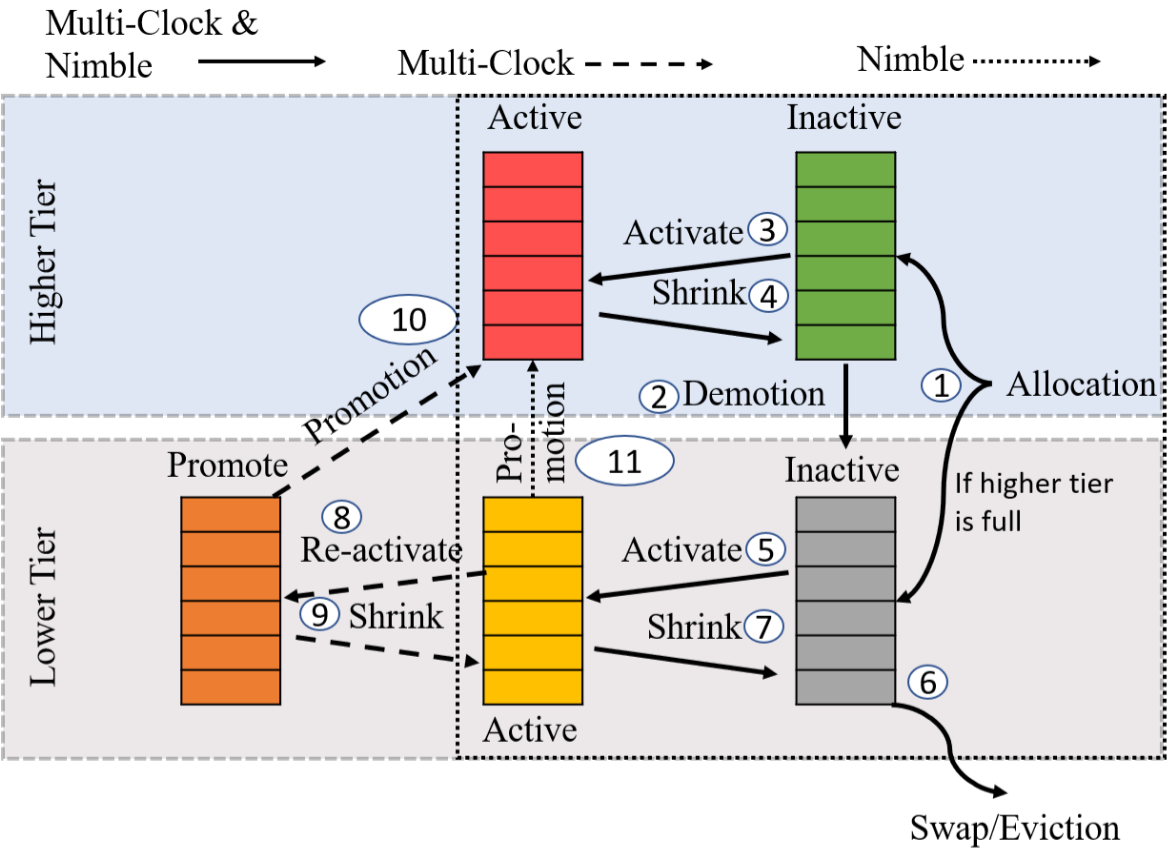
\includegraphics[scale=0.21]{multiclock addition.png}
    \caption{Multi-Clock additions over other methods of tiering.}
\end{figure}

\subsection{Linux Kernel}

The Linux operating system’s (OS) kernel combines the features of multiple policies to catch both general and edge cases.  The meshed policies include features used in Clock Pro, an improvement on LRU which attempts to also track frequency [9], for file-backed pages and LRU 2Q, the split-list approach mentioned above, with aspects of least frequently used (LFU) [7].  In general, Linux is considered as using LRU 2Q.  The kernel attempts to keep file-backed and anonymous pages in active use by a process in the active list, and pages not used by a process in the inactive list [8].  Pages in the inactive list have been unmapped from the space of the process using them, requiring a soft page fault to bring them back to the active list if again needed.  File-backed pages are initially moved to the inactive list, with the assumption that a process will only need the contents once, only moving them to the active list if accessed twice. 

Unlike the basic approach, Linux does not keep structured lists specific to LRU or FIFO.  Instead, it uses circular lists scanned like in Clock (6).  There is no need to sort either list, freeing up considerable resources.  A daemon simply runs on a cadence to scour the lists for pages needing moved between them or between tiers (or simply evicted). 

Many of these strategies to improve basic algorithms involve balancing the sizes of different lists or finding ways to track frequency as well as recency to know whether to add a needed page directly to the active list or if the kernel is already doing a good job.  So far, these strategies and techniques have involved clever use of algorithms and data structures, but there is another world to consider.  This other world allows for specialization for given tasks or use cases and can learn to elegantly optimize memory management well beyond the realm of manual human design: machine learning and deep learning! 

\section{Machine Learning Algorithms}

Machine learning accomplishes the training of new, better optimized policies than the more basic approaches to memory management.  Given a purpose or dataset, an ML solution can be tuned for striking efficiency in specific use cases.  Techniques can involve supervised learning, reinforcement learning, “punishing” bad behavior, and mathematical concepts like support vector machines (SVMs), random forests, k-nearest neighbors, and Baye’s theorem.  Benefits are evident in reducing the time needed to process given data, increasing the overall amount of data or instructions runnable through memory or CPUs (throughput), and even in maximizing the battery life of mobile devices or reducing power consumption of large data crunching centers [10]. 

\subsection{Hardware-Aware Machine Learning: Modeling and Optimization}
Computation speed can be increased and energy consumption decreased significantly at the cost of a small percentage of accuracy in ML models.  Multiple methods achieve some success by pruning unnecessary hyperparameter-heavy layers of deep neural nets (DNNs) or reducing the bit width per multiply-accumulate operation [12].  These solutions are effective, but difficult to port to other architectures.  Diana Marculescu, Dimitrios Stamoulis, and Ermao Cai of Carnegie Mellon University have formulated a more effective solution by focusing on ML based on Bayesian optimization and neural architecture search to produce hardware-aware runtime and energy modeling.  Their methodologies involve hyperparameter tuning given feedback from building and running deep learning (DL) algorithms using surrogate functions which are easier to calculate than the actual DL functions. 

\subsection{Machine Learning-Based Cache Replacement Policies: A Survey}
Long short-term memory (LSTM) are neural networks using sequential data to predict the output of the next time step [13].  For example, a history of cache accesses can be the sequential data.  The net can either adjust its own weights or track rewards and/or punishments in deciding on the path to follow in self-adjustment of the optimized policy.  LeCAR is an ML take on CAR designed for small cache sizes relative to the workload which exploit LRU and LFU.  Each of the LRU and LFU have probability-distributed weights, and each time something from the FIFO queue cache history is brought back to the cache, the weights are altered in a reinforced learning, regret-style dynamic.  If the returned entry was evicted by LRU, LFU’s weight is adjusted to be more likely to be used, next time, and visa versa.  Basically, it regrets having not followed the other algorithm. 

Similar to LeCAR, CACHEUS uses scan and churn data, or cache entries which are accessed only once versus entries accessed repeatedly with equal probability, with much the same techniques as LeCAR.  Instead of LFU and LRU, it uses scan-resistant LRU (SR-LRU) and churn-resistant LFU (CR-LFU). 

\subsection{FlexMem Adaptive Page Profiling and Migration}
FlexMem is a tool for transparent tiered memory management which uses both performance counter-based and fault-based profiling methods to overcome the inflexibility of previous page profiling methods [14].  FlexMem claims better identification of warm pages and a better facilitation of demotion of pages in higher tiers to make room for ready-to-promote pages in lower tiers.  In older or more traditional tools, pages promotions may be limited by how much free space there is in a higher tier (such as in MEMTIS) or a more aggressive reclamation approach may be taken on the higher tier (like with MTM and Unimem), leading to higher migration overhead.   

A unique way of estimating page access frequency is to count the number of NUMA hinting faults from page profiling, minor faults caused each time the kernel tries to access a page’s information, forcing the \_PAGE\_PROTNONE bit to be temporarily set.  Relying on NUMA hinting faults can be expensive, however, so enter performance counters.  Performance counters are special CPU registers able to be set up to count specific events, such as processor event-based sampling (PEBS).  Upon sampling retired store instructions or last-level cache (LLC) misses, the virtual memory address targeting the sampled events is recorded, providing metadata such as page access counts. 

During tests between TPP (using minor faulting) and MEMTIS (using performance counters) on different workloads, it was shown that neither was a clear winner, so the authors of FlexMem decided to hybridize both. 

\subsection{IDT Intelligent Data Placement for Multi-tiered Main Memory}
IDT, Intelligent Data Placement for Multi-Tiered Main Memory, employs reinforcement learning to better adjust page demotion criteria and predict pages to promote to faster tiers [15].  Its specialty is its testing in a four-tiered memory setup with all four tiers available to the kernel as main memory, while using only lightweight ML solutions for prediction. 

\subsection{Tiered Memory Management: Access Latency is the Key!}
Midhul Vuppalapati and Rachit Agarwal created the Colloid design based on monitoring access latency between memory tiers [16].  Most ML designs focus on placing as many hot pages in the fastest tier as possible, keeping warm pages in secondary tiers, and finally colder pages in the slowest tiers.  In realistic conditions, this can lead to the otherwise fastest tier suddenly having a slower access time because of faster tiers’ bandwidth being taken by transfers and accesses.  Colloid offers an intelligent remedy by tracking access latencies based on already-used bandwidth of tiers, utilizing normally slower tiers where appropriate and where it would make sense. 

\subsection{TieredMMS: A Modular Tiered Memory Management System}
TieredMMS is modular and hardware based [17].  Its creators designed it to track page allocation and release in user space to count accesses and allocate the hottest pages to DRAM.  Page heat is determined by access frequency, but the product still utilizes the Linux OS’s recency-based LRU lists for simplicity.  Hot and cold pages are placed in a ring buffer shared by user and kernel spaces, using warm pages between to keep hot and cold from migrating too much.  TieredMMS moves hot pages to the active list and cold pages to the inactive list.  It uses two watermark levels.  The high watermark triggers an attempt to remove cold pages from the inactive list and move them to lower tiers, while if free memory falls below the low watermark, special threads—demotion threads on DRAM nodes and promotion threads on other nodes—are woken to speed things along. 

\subsection{Learning-Based Page Replacement Scheme for Efficient I/O Processing}
Hwajung Kim developed an approach to memory management using both LRU and most recently used (MRU) algorithms, using reinforcement learning to minimize the regret of having not chosen the better algorithm in a given situation.  It is called Learning-based Page Replacement, or LPR.  It analyzes access patterns and probabilistically calculates explorative options in each situation, as well as exploiting currently known options.

\section{How Machine Learning Algorithms Compare}
In hardware-aware deep learning optimizations, HyperPower outperforms hardware-unaware Bayesian models by 350\% and NeuralPower is 70\% more accurate in predicting convolutional neural net (CNN) power and runtime needs over the next-best competitor, Paleo. 

Between LeCAR and CACHEUS, LeCAR is designed for LRU and LFU-friendly datasets while CACHEUS is made for scan and churn-friendly datasets.  When tested on webmail workloads, CACHEUS proved to be the most consistent algorithm, outperforming LeCAR 43.95\% to 42.08\%. 

FlexMem is evaluated with representative memory-intensive applications and compared against Tiering-0.8, TPP, MEMTIS.  The latter three are outperformed by a geomean of 28\% (32\%, 23\%, 27\%, respectively, across all workloads overall).  FlexMem reduces page migration failure by 25\% and improves fast memory usage by 21\%. 

IDT performs 208\% better than the default Linux kernel and 11.2\% better than other ML solutions. 

For TieredMMS, the memory-intensive workloads of Liblinear and Graph500 are chosen for testing and comparisons.  When used along with Linux’s default tiered memory management system, AutoNUMA, TieredMMS improves performance by up to 397\%.  When compared to Memtis, TieredMMS outperforms by anywhere from 8\%-26.3\% in half the test cases. 

LPR was tested with scientific and graph processing applications and in real-world scenarios, reduces execution time by 62\% on out-of-core graph processing. 

\section{Conclusion}
Computers have been used with great success to improve the lives of humanity, and the algorithms governing their inner workings have grown to mountainous heights over the last eighty years.  Many different tools and techniques have been developed to that end, including even helping computers think like humans.  Different tools have different areas of focus and differing means of achieving even the same ends.  Some work in kernel space, and some in user space.  Some are only for big data science, and some specialize in saving time or money.

\section*{Acknowledgment}
I can't thank my professor, Rahul Dubey, enough.  He has worked very hard to ensure that all his students have ample understanding of research, computer science, and how to write academic papers using the Latex document writing language.  While I chose to pursue a different specialty, he also made explainable artificial intelligence sound very fun and useful.

\begin{thebibliography}{00}
\bibitem{b1} R. Sheldon, G. Kranz, D. Raffo, ``Tiered storage,'' TechTarget, Last updated September 2021, Last accessed 4 May 2025, [Online] Available: \url{https://www.techtarget.com/searchstorage/definition/tiered-storage#:~:text=IBM%20pioneered%20the%20multi%2Dtiered,Attachment%20(SATA)%20hard%20drives.}.
\bibitem{b2} ``Hierarchical storage management,'' Wikipedia, Last edited 25 February 2025, Last accessed 4 May 2025, [Online] Available: \url{https://en.wikipedia.org/wiki/Hierarchical_storage_management}.
\bibitem{b3} A. Huffman, 23 January 2013, ``NVM Express,'' Revision 1.0e, Page 2, Last accessed 4 May 2025, [Online] Available: \url{https://nvmexpress.org/wp-content/uploads/NVM-Express-1_0e.pdf}.
\bibitem{b4} ``Solid-state drive,'' Wikipedia, Last edited 1 May 2025, Last accessed 4 May 2025, [Online] Available: \url{https://en.wikipedia.org/wiki/Solid-state_drive#:~:text=SSDs%20using%20Flash,-SSD%20evolution&text=Flash%20memory%2C%20a%20key%20component,MB%20SSD%20for%20IBM%20laptops.}.
\bibitem{b5} H. Al Maruf, H. Wang, A. Dhanotia, J. Weiner, N. Agarwal, P. Bhattacharya, C. Petersen, M. Chowdhury, S. Kanaujia, P. Chauhan, ``Different-tiers-has-different-characteristics-with-varied-memory-access-latency-in-a,'' 6 June 2022, [Online] Available: \url{https://www.researchgate.net/publication/361162182/figure/fig1/AS:1164536778358786@1654658612492/Different-tiers-has-different-characteristics-with-varied-memory-access-latency-in-a.png}.
\bibitem{b6} R. Battle, ``Machine learning feature selection for tuning memory page swapping,'' September 2013, [Online] Available: \url{https://calhoun.nps.edu/server/api/core/bitstreams/5c6b626c-d9d5-4a80-b990-669272624afc/content}.
\bibitem{b7} sourcejedi, ``What page replacement algorithms are used in Linux kernel for OS file cache?,'' Unix \& Linux Stack Exchange, Last edited 5 November 2018, [Online] Available: \url{https://unix.stackexchange.com/questions/281974/what-page-replacement-algorithms-are-used-in-linux-kernel-for-os-file-cache}.
\bibitem{b8} J. Corbet, ``Better active/inactive list balancing,'' LWN.net, 2 May 2012, [Online] Available: \url{https://lwn.net/Articles/495543/}.
\bibitem{b9} J. Corbet, ``A CLOCK-Pro page replacement implementation,'' LWN.net, 16 August 2005, Last accessed 4 May 2025, [Online] Available: \url{https://lwn.net/Articles/147879/}.
\bibitem{b10} D. Marculescu, D. Stamoulis, E. Cai, ``Hardware-aware machine learning: modeling and optimization,'' 14 September 2018, [Online] Available: \url{https://arxiv.org/pdf/1809.05476}.
\bibitem{b11} A. Maruf, A. Ghosh, J. Bhimani, D. Campello, A. Rudoff, R. Rangaswami, ``MULTI-CLOCK: Dynamic Tiering for Hybrid Memory Systems,'' 2022, [Online] Available: \url{https://users.cs.fiu.edu/~raju/WWW/publications/hpca2022/paper.pdf}.
\bibitem{b12} P. Pratheeksha, S.A. Revathi, ``Machine learning-based cache replacement policies: a survey,'' International Journal of Engineering and Advanced Technology (IJEAT), Volume-10 Issue-6, August 2021, [Online] Available: \url{https://www.ijeat.org/wp-content/uploads/papers/v10i6/F29070810621.pdf}.
\bibitem{b13} D. Xu, J. Ryu, J. Baek, K. Shin, P. Su, D. Li, ``FlexMem adaptive page profiling and migration,'' 2024, [Online] Available \url{https://pasalabs.org/papers/2024/ATC24_FlexMem.pdf}.
\bibitem{b14} J. Chang, W. Doh, Y. Moon, E. Lee, J.H. Ann, ``IDT intelligent data placement for multi-tiered main memory,'' The 33rd International Symposium on High Performance Parallel and Distributed Computing (HPDC ’24), June 2024, [Online] Available: \url{https://dl.acm.org/doi/pdf/10.1145/3625549.3658659}.
\bibitem{b15} M. Vuppalapati, R. Agarwal, ``Tiered memory management: acces latency is the key!,'' ACM SIGOPS 30th Symposium on Operating Systems Principles (SOSP ’24), November 2024, [Online] Available: \url{https://www.cs.cornell.edu/~midhul/papers/colloid.pdf}.
\bibitem{b16} S. Wei, M. Ren, C. Jia, G. Wang, L. Yue, X. Zhong, H. Chen, ``TieredMMS: a modular tiered memory management system,'' 2024, [Online] Available:\url{https://www.msstconference.org/MSST-history/2024/Papers/msst24-6.2.pdf}.
\bibitem{b17} H. Kim, ``Learning-based page replacement scheme for effective I/O processing,'' 8 February 2025, Sci Rep 15, 4721 (2025), [Online] Available: \url{https://doi.org/10.1038/s41598-025-88736-4}
\end{thebibliography}

\end{document}
